\section{Операторы(Statements)} 
\subsection{AST, операторы, трасса выполнения программы}
Система {\sf Symbalg} является инструментом для кодогенерации. Как правило, код программыё на каком-либо языке программирования (в нашем случае используется язык {\sf C++}) состоит из модулей и написанного внутри них текста программы. 

\begin{center}
    \begin{figure}
        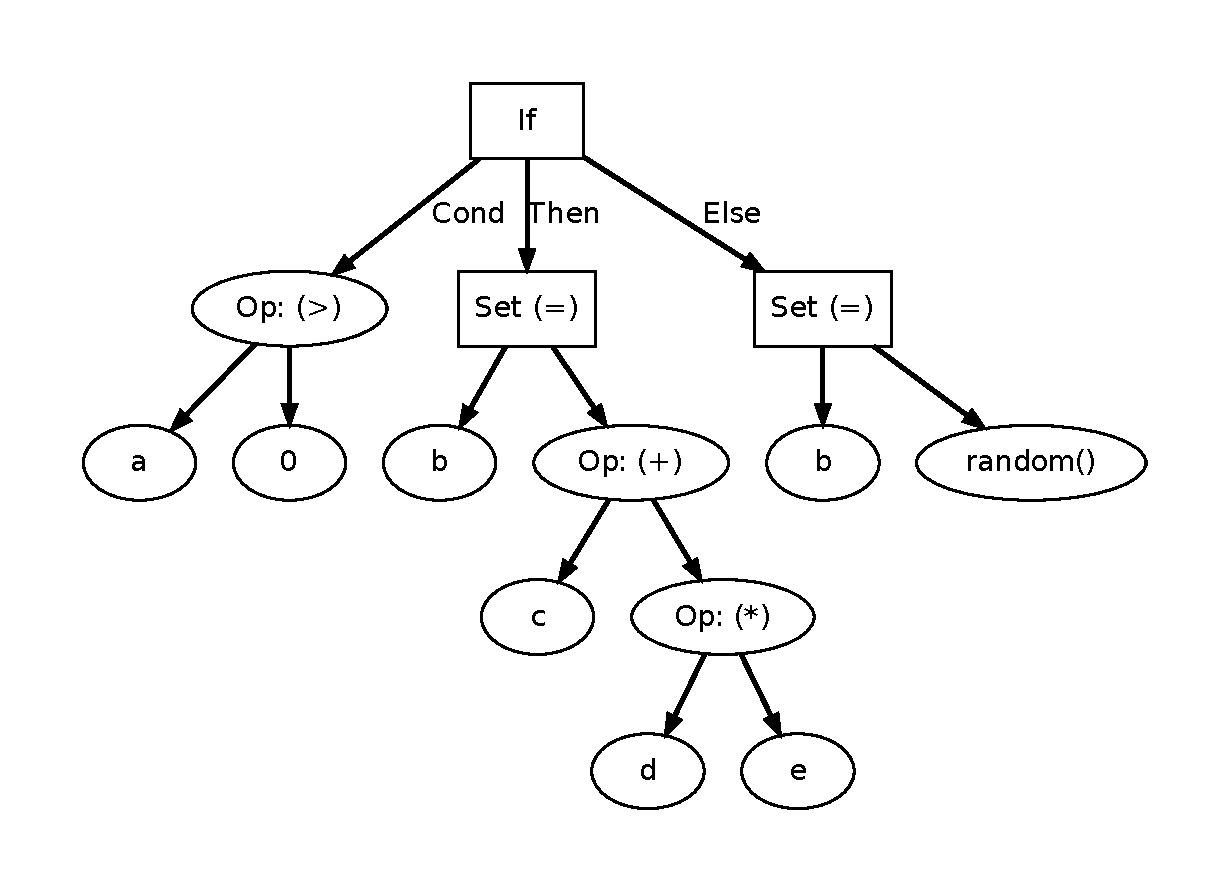
\includegraphics[width=\textwidth]{images/If.pdf}
        \caption{Пример AST}
        \label{fig:ast}
    \end{figure}
\end{center}

Программный код на языке {\sf C++} представим в виде AST (Abstract Syntax Tree~--- Абстрактное синтаксическое дерево).
AST программного кода~--- дерево, узлами которого являются операторы языка программирования или операции, а листьями~--- операнды (рис.\ref{fig:ast}). Реализация операций и операндов уже описана в прошлой главе~(\ref{sec:AST}). В этой главе рассмотрим реализацию операторов языка программирования {\sf C++}.

Оператор в императивных языках программирования (коим является {\sf C++})~--- это наименьшая автономная часть языка программирования; команда. В таблице~\ref{tab:stms} приведены примеры различных операторов на языке {\sf C++}.
\begin{table}
    \begin{center}
        \begin{tabular}{|l|l|}
            \hline
            Оператор & Пример\\
            \hline
            Объявление & \verb"int a = 0;"\\
            \hline
            Присваивание & \verb"a = b + c;" \\
            \hline
            Последовательность операторов & \verb"int a;" \\
                                          & \verb"a = b + c;"\\
            \hline
            Блок операторов &\verb"{" \\
                            &\verb"    int a;" \\
                            &\verb"    a = b + c;"" \\
                            &\verb"}" \\
            \hline
            Условный оператор & \verb"if (a != b){" \\
                              & \verb"    d = c + 1;" \\
                              & \verb"} else {" \\
                              & \verb"    d = c + 2;" \\
                              & \verb"}"\\
            \hline
            Оператор переключения & \verb"switch (a){" \\
                                  & \verb"    case 0:" \\
                                  & \verb"        d = c + 1;" \\
                                  & \verb"        break;" \\
                                  & \verb"    case 1:" \\
                                  & \verb"        d = c + 2;" \\
                                  & \verb"        break;" \\
                                  & \verb"}"\\
            \hline
            Цикл For & \verb"for(int i = 0; i < N; ++i){" \\
                     & \verb"    d+=i;" \\
                     & \verb"}" \\
            \hline
            Цикл с предусловием & \verb"while (a<10){" \\
                                & \verb"    a++;" \\
                                & \verb"}" \\
            \hline
            Цикл с постусловием & \verb"do {" \\
                                & \verb"    a++;" \\
                                & \verb"while (a<10);" \\
            \hline
            Вызов подпрограммы & \verb"IncreaseTemp(10);" \\
            \hline
            Возврат из подпрограммы & \verb"return 0;"\\
            \hline
        \end{tabular}
    \end{center}
    \caption{Различные виды операторов языка {\sf C++}}
    \label{tab:stms}
\end{table}

Хоть AST~--- дерево, набор операторов также представим в виде последовательно идущего программного кода~--- трассы выполнения программы. Это наиболее привычный вид, который используется при написании программы человеком~--- последовательно строчку за строчкой добавлять операторы в трассу выполнения программы. Этот принцип взят за основу кодогенерации в системе {\sf Symbalg}. 

Система {\sf Symbalg} реализована на языке программирования {\sf Python}, и используется в рамках синтаксиса языка {\sf Python}. Соответственно все использование системы должно вестись в рамках синтаксиса языка {\sf Python}, не используя дополнительные файлы с псевдокодом, и ограничивая использование строковых конструкций. {\sf Python}~--- объектно-ориентированный язык программирования, и все сущности представляют собой объекты~--- экземпляры классов. Операторы реализованы как классы языка {\sf Python}, и их экземпляры можно создавать при помощи явного использования конструкторов. Этот метод создания AST, несомненно, является громоздким и нежелательным. Для создания AST путем наполнения трассы выполнения программы были сформулированы следующие постулаты, на которых основана идеология системы кодогенерации:

\begin{enumerate}
    \item Хранение AST в виде дерева, узлами и листьями которого являются экземпляры классов системы {\sf Symbalg}.
    \item Возможность создания дерева с нуля, наполняя трассу выполнения программы в рамках синтаксиса языка {\sf Python}.
    \item Возможность гибко работать с уже созданным фрагментом AST, как с традиционным деревом (создание нового дерева на основе существующего(их), добавление ветвей, замена ветвей, удаление ветвей, рекурсивный перебор всех элементов дерева и т.д.).
\end{enumerate}

Опишем реализацию сформулированных постулатов по пунктам.

\subsection{Иереахия классов, реализующих операторы}

Базовым классом для операторов является \verb"BaseStm" и основная логика операторов описана в модуле \verb"statement.py". 
На рисунке~\ref{fig:hier} представлены классы, которые реализуют поведение операторов.

\begin{center}
    \begin{figure}
        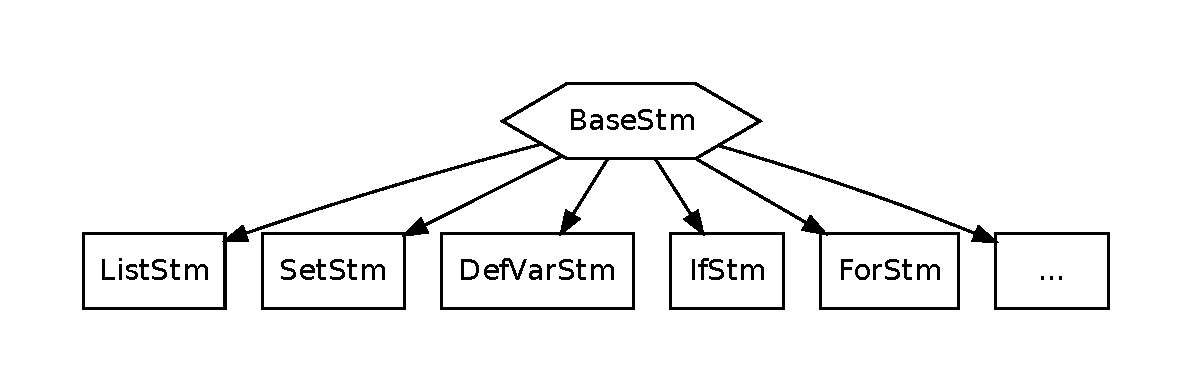
\includegraphics[width=\textwidth]{images/Hier.pdf}
        \caption{Иерархия классов, реализующих операторы}
        \label{fig:hier}
    \end{figure}
\end{center}

Каждый наследник класса \verb"BaseStm" реализует один из операторов, приведенных в таблице~\ref{tab:stms}. В таблице~\ref{tab:clstms} представлено сопоставление операторов и классов, их реализующих.
\begin{table}
    \begin{center}
        \begin{tabular}{|l|l|l|}
            \hline
            Оператор & Класс, реализующий                   & Описание класса\\
                     & оператор                             &\\
                                                           &&\\         
            \hline
            Объявление & \verb"DefVarStm"                   &Имеет поля \verb"name", \verb"type" и \verb"value"\\
            \hline
            Присваивание & \verb"SetStm"                    &Имеет поля \verb"lvalue", \verb"op" и \verb"expr"\\
            \hline
            Последовательность & \verb"ListStm"             &Имеет поле \verb"_list"~--- список операторов\\
            операторов         &                            &\\
            \hline
            Блок операторов &\verb"Пока не реализован"      &\\
            \hline
            Условный оператор & \verb"IfStm"                &Имеет поля \verb"cond", \verb"mode", \verb"_then" и \verb"_else"\\
                                                           &&Может работать в двух режимах: \\         
                                                           &&1) Только ветвь True (\verb"mode==True"),   \\         
                                                           &&2) Ветвь True и одна ветвь Else (\verb"mode==False"),   \\         
            \hline
            Оператор     & \verb"Пока не реализован"        &\\
            переключения &                                  &\\
            \hline
            Цикл For & \verb"ForStm"                        &Имеет поля \verb"init", \verb"cond", \verb"step" и \verb"code"\\
            \hline
            Цикл с предусловием & \verb"Пока не реализован" &\\
            \hline
            Цикл с постусловием & \verb"Пока не реализован" &\\
            \hline
            Вызов подпрограммы & \verb"Пока не реализован"  &\\
            \hline
            Возврат из   & \verb"Пока не реализован"        &\\
            подпрограммы &                                  &\\
            \hline
        \end{tabular}
    \end{center}
    \caption{Различные виды операторов языка {\sf C++}}
    \label{tab:clstms}
\end{table}

Эта иерерахия и лежит за реализацией первого пункта постулатов из трех.

\subsection{Заполнение AST путем наполнения трассы выполнения программы}
Второй постулат заключается в том, чтобы существовала возможность создания AST путем набирания трассы выполнения кода программы на языке {\sf C++} в рамках синтаксиса языка {\sf Python}. 
Первое, на чем нужно условиться, это то, что участок AST представляется в системе {\sf Symbalg}, как экземпляр класса \verb"ListStm".
Таким образом, в системе {\sf Symbalg}, наполнение трассы выполнения программы заключается в формировании списка операторов, который хранится в экземпляре класса \verb"ListStm".

Для этого функционала нам нужно по особому обрабатывать код на языке {\sf Python}, который будет составлять желаемый участок AST. 
Такая обработка кода в системе {\sf Symbalg} достигается путем исполнения участка кода на языке {\sf Python} в искусственно созданном пространстве имен. 

В этом пространстве имен нам хотелось бы легко вводить участок AST, то есть:
\begin{itemize}
    \item Использовать переменные внутри выражений без их изначального инициализирования
    \item Позволить вводить некоторые специфичные для языка {\sf C++} конструкции (циклы For, i++ и т.д) в синтаксисе языка {\sf Python}
    \item Просто вводить AST как программный код без самостоятельного создания каких-либо объектов.
\end{itemize}

Для этого предлагается реализовать класс, эмулирующий пространство имен~--- \verb"NamespaceStm".
Чтобы выполнить некий фрагмент кода в нужном пространстве имен, нужно этот фрагмент кода в виде строки передать в процедуру 
\verb"exec", а также в качестве локального пространства имен передать нужное нам пространство имен.
Для того, чтобы это можно было сделать, для этого класса, реализующего пространство имен нужно создать методы \verb"__getitem__" и \verb"__setitem__", которые используется в традиционных пространств имен (обычные словари) для возврата элемента по имени. 
Тем самым, вместо возврата элемента словаря в методе \verb"__getitem__" мы можем обрабатывать пришедшую на вход строку как угодно и совершать любые действия. Метод \verb"__setitem__" вызывается при конструкциях типа:
\begin{verbatim}
a = ...  # вызовет .__setitem__("a")
\end{verbatim}
Будем различать несколько типов переменных во фрагменте кода, представляющего участок AST:
\begin{itemize}
    \item переменная \verb"_"~--- при встрече с такой переменной создастся экземпляр класса \verb"EmptyVar".
    \item переменная, начинающаяся со знака подчеркивания~--- переменная, которая не войдет в AST и используется как обычная переменная языка {\sf Python}.
    \item переменная, не начинающаяся со знака подчеркивания~--- для нее создастся (если уже не был создан) экземпляр класса \verb"var".
    \item зарезервированная {\sf Symbalg} переменная для написания некоторых операторов (например~--- \verb"For", \verb"If", ...). При их встрече в коде, происходит создание экземпляра класса соответствующего оператора.
\end{itemize}

Для того, чтобы реализовать описанный функционал, был реализован декоратор \verb"@statement". При декорации им метода, все, что является телом этого метода передается в виде строки в процедуру \verb"exec" с локальным пространством имен \verb"NamespaceStm". 

Пример создания участка AST при помощи метода, декорируемого декоратором \verb"@statement":
\begin{verbatim}
@statement
def test():
    a[0,1,2] = w//b[2,3]
    For[i:0,N]
    a[1,3,4] = g[1,2,3]
\end{verbatim}

При вызове полученной функции возвращается экземпляр класса \verb"ListStm", с именем \verb"test". При вызове этого метода в качестве именованных аргументов можно передавать пары "переменная" : "операция". При этом во всем участке AST совершится подстановка предложенной операции вместо предложенной переменной.

В таблице~\ref{tab:examstms} приведены примеры использования операторов языка {\sf C++} внутри функций, декориуемых декоратором \verb"@statement".

\begin{table}
    \begin{center}
        \begin{tabular}{|l|l|}
            \hline
            Оператор & Пример\\
            \hline
            Объявление & \verb"В явном виде не реализован"\\
            \hline
            Присваивание & \verb"a = 1" \\
                         & \verb"----------------------------------------------" \\
                         & \verb"b += 1" \\
            \hline
            Последовательность операторов & \verb"a = 1" \\
                                          & \verb"b += 1" \\
            \hline
            Блок операторов &\verb"Пока не реализован" \\
            \hline
            Условный оператор & \verb"If[a>b]"\\
                              & \verb"c+=1"\\
                              & \verb"Else"\\
                              & \verb"c+=2"\\
                              & \verb"End"\\
            \hline
            Оператор переключения & \verb"Пока не реализован"\\
            \hline
            Цикл For & \verb"For[counter:start, stop]" \\
                     & \verb"B += counter"\\
                     & \verb"End"\\
                     & \verb"----------------------------------------------" \\
                     & \verb"For[counter:start, stop, step]"\\
                     & \verb"B /= counter"\\
                     & \verb"End"\\
                     & \verb"----------------------------------------------" \\
                     & \verb"For[counter, start, condition, nextstep]"\\
                     & \verb"B += counter"\\
                     & \verb"End"\\
                     & \verb"----------------------------------------------" \\
                     & \verb"For[type, counter, start, condition, nextstep]"\\
                     & \verb"B += counter"\\
                     & \verb"End"\\
            \hline
            Цикл с предусловием & \verb"Пока не реализован" \\
            \hline
            Цикл с постусловием & \verb"Пока не реализован" \\
            \hline
            Вызов подпрограммы & \verb"Пока не реализован" \\
            \hline
            Возврат из подпрограммы & \verb"Пока не реализован"\\
            \hline
        \end{tabular}
    \end{center}
    \caption{Пример реализации операторов языка {\sf C++}}
    \label{tab:examstms}
\end{table}

\subsection{Работа с AST как с деревом}
С участком AST(экземпляром класса \verb"ListStm") можно совершать различные действия. Для класса \verb"ListStm" определено сложение, которое интерпретируется как послеследование одного участка AST за другим. Уже существующий экземпляр класса \verb"ListStm" можно использовать как внутри пространства имен \verb"NamespaceStm", так и вне его. Использовать внутри \verb"NamespaceStm" можно при помощи следующей конструции:
\begin{verbatim}
_[StmName()] 
\end{verbatim}
При обращении к оператору, в круглых скобках можно указывать аргументы. При их помощи можно совершать изменения в AST, которое интерпретируется этим оператором. Есть два различных вида аргументов:
\begin{itemize}
    \item именованные аргументы, передаваемые при вызове экземпляра класса \verb"ListStm", используемые для макроподстановок. Например конструкция:
    \begin{verbatim}
StmName(a=b)
    \end{verbatim}
заменит все переменные \verb"a" внутри AST на переменную \verb"b"
    \item именованный аргумент \verb"_conv=func"~--- позволяет рекурсивно применять метод \verb"func" ко всем узлам AST. Метод может как собирать информацию с AST, так и изменять его части. Пример рекурсивной функции и ее применения:
    \begin{verbatim}
def offset_1(x):
    if isinstance(x, IndexOp) and type(x.b) is tuple:
        x.b = tuple([i+1 for i in x.b])
    return x

print StmName()(_conv=offset_1)    
    \end{verbatim}
    Эта функция прибавляет единицу ко всем, встречающимся в AST, индексам (содержимым квадратных скобок)
\end{itemize}
\[
    
\]